Traditionally, in the context of relativistic heavy-ion physics, proton-nucleus collisions were considered as a benchmark to investigate Cold-Nuclear-Matter (CNM) effects in the absence of a deconfined medium, which on the contrary one supposes to be produced in the nucleus-nucleus case. However, recent experimental results led people to partially reconsider such a paradigm. 
In particular, the study of soft observables in high-multiplicity \pPb (and even pp) collisions led to the observation of signals qualitatively, and often also quantitatively, very similar to the ones measured in nucleus-nucleus collisions and traditionally attributed to the formation of a hot deconfined medium displaying a collective behaviour: long-range azimuthal 2-particle correlations~\cite{Khachatryan:2010gv,CMS:2012qk,Abelev:2012ola,Aad:2012gla}, non-vanishing flow harmonics~\cite{ABELEV:2013wsa,Khachatryan:2015waa}, increasing baryon/meson ratio as a function of $\pT$~\cite{Abelev:2013haa}, enhancement of strange-hadron production~\cite{Adam:2015vsf}. Many authors interpreted these observations as indications that the same strongly-interacting medium, with a collective hydrodynamic expansion driven by pressure gradients, supposed to be formed in nucleus-nucleus collisions is also produced in the case of small systems. If the hydrodynamic scheme provides a consistent framework capable of describing essentially all the above observations, its strong underlying assumptions, i.e. the realization of a system not too far from local thermal equilibrium with a mean-free-path much smaller than its size ($\lambda_{\rm mfp}\ll L$), looks challenging to satisfy for the case of small systems like the ones produced in proton-nucleus collisions. Hence, some authors looked for alternative interpretation of the data -- in particular the ones related to particle correlations and flow harmonics -- in terms, for instance, of initial-state effects (Color-Glass-Condensate~\cite{Dusling:2013qoz}), of the formation of a system with small parton-parton cross-sections~\cite{Bzdak:2014dia} or of quantum-mechanical interference in the presence of multiple sources of particle production, entailing to reconsider the no-interaction baseline before looking for final-state collective effects~\cite{Blok:2017pui}.

On the other hand, no signature of jet-quenching or suppression of high-$\pT$ particle production was observed in high-multiplicity proton-nucleus collisions~\cite{Acharya:2018qsh}.  At first glance this may look in contradiction with the interpretation of the  measurements involving soft observables in terms of non-trivial final-state medium effects. One should in any case consider that the quenching of jets due to parton energy-loss in the QGP has a strong dependence on the thickness of the crossed matter (one has $\Delta E\sim \alpha_s\hat q L^2$ for the average energy-loss due to medium-induced gluon radiation). On the contrary, if one accepts the hydrodynamic paradigm, the smaller size of the medium with respect to the nucleus-nucleus case would lead to even larger initial pressure gradients and hence to a larger collective acceleration of the fluid, able to compensate its shorter lifetime. Hence, although reproducing within a unified theoretical framework the apparently opposite observations in the low-$\pT$ and high-$\pT$ sectors looks challenging, the latter are not necessarily in contradiction.

In light of the above findings, as an independent probe, it is clearly of interest to address the study of small systems also through heavy-flavour observables. Due to their large mass c and b quarks are in fact produced in the very first instants in hard processes described by pQCD, at most affected by nuclear modifications of the Parton Distribution Functions (nPDFs) and by an initial transverse-momentum broadening acquired in CNM. %Since the large mass suppresses also the excitation of $Q\bar Q$ pairs from the vacuum during hadronization, any detected heavy-flavour hadron certainly carries a $c$ or $b$ quark produced during the initial collision and which has crossed the produced medium. 
It looks then natural to extend transport calculations, developed to describe heavy-flavour propagation through the plasma formed in nucleus-nucleus collisions, also to the case of small systems, assuming as a working hypothesis that also in this case a hot deconfined medium is formed. The theoretical modelling involves the same processes as in the heavy-ion case: the so-called CNM effects (nPDFs and initial $k_{\rm T}$-broadening) modifying the hard $Q\overline{Q}$ production, the propagation of the heavy quarks throughout the fireball and finally their hadronization in the presence of a hot medium. The only difference is that, in the case of small systems, it is mandatory to include event-by-event fluctuations in the initial conditions.

\begin{figure}[ht]
\centering
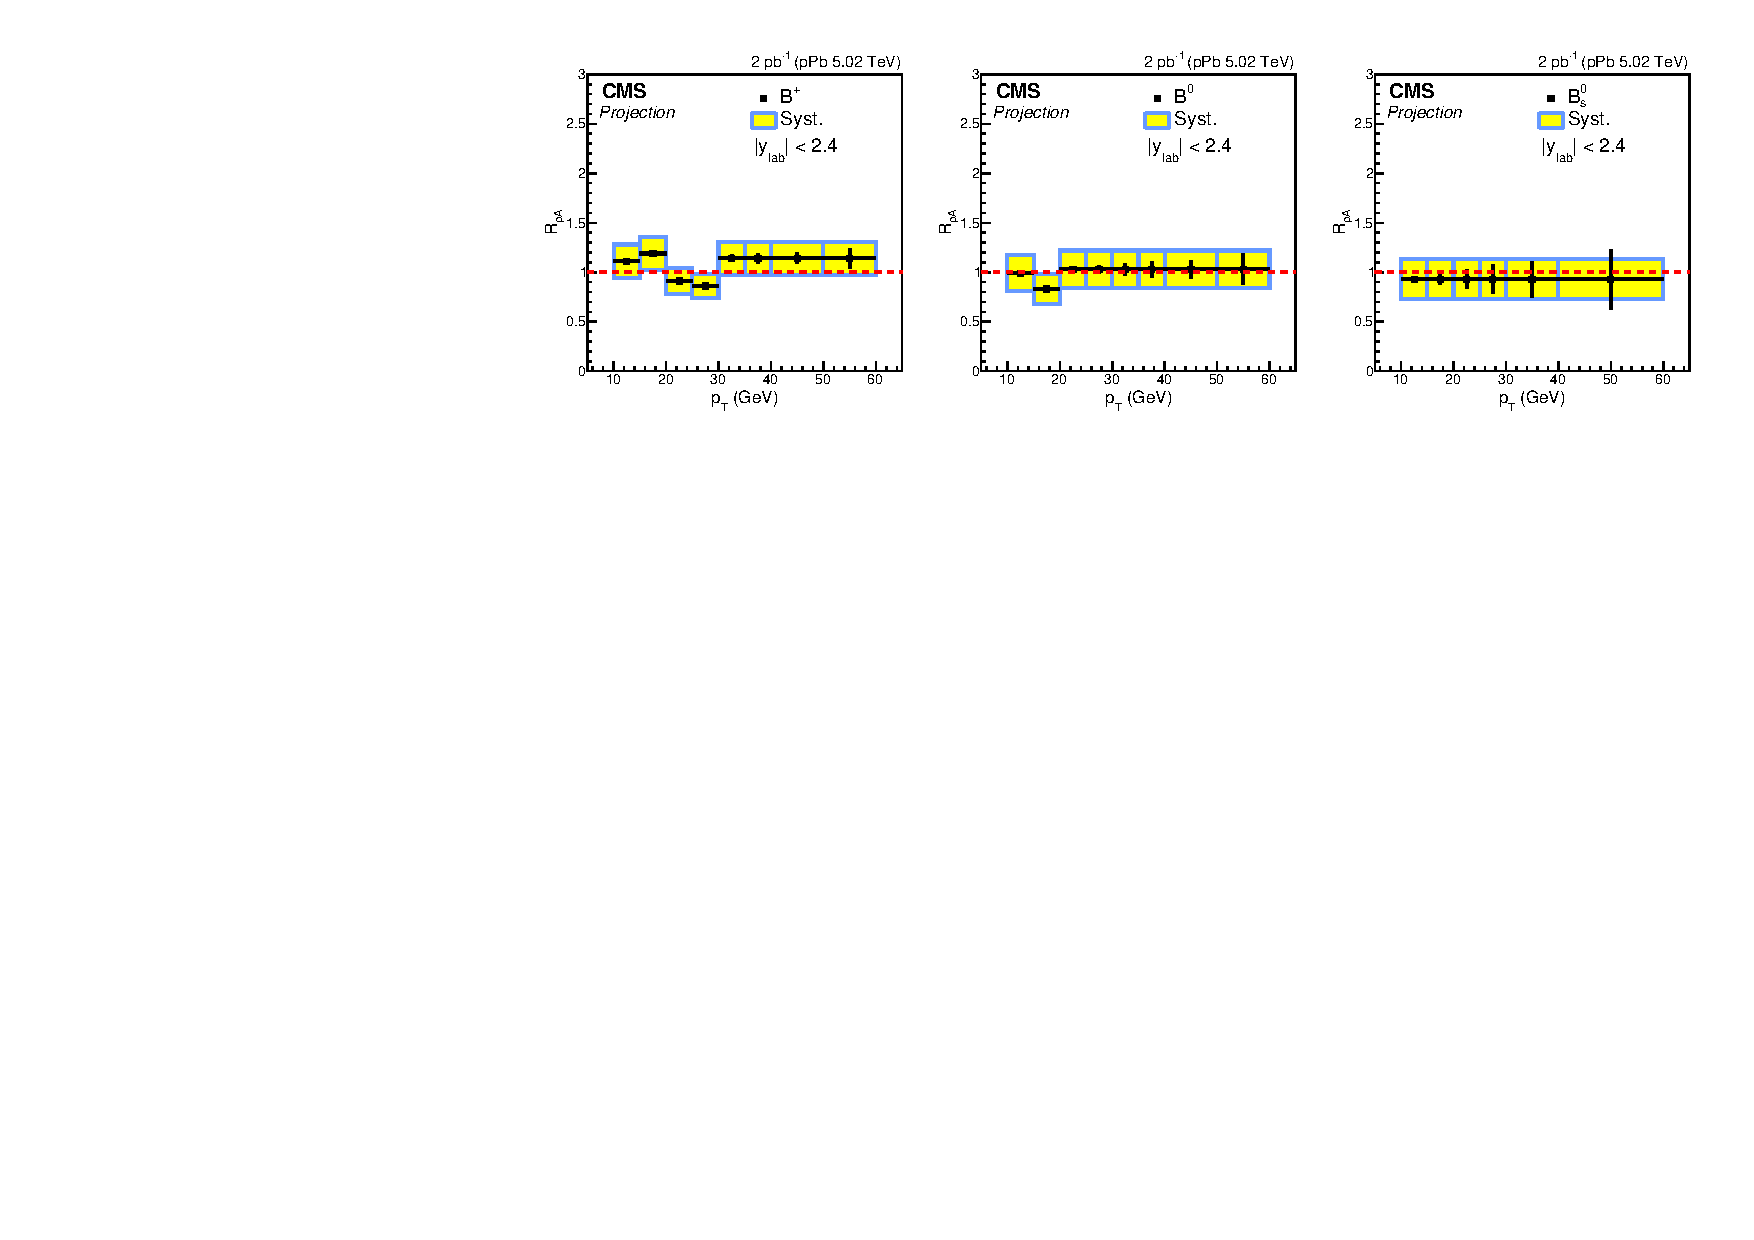
\includegraphics[trim=0 0 13cm 0,clip,width=0.42\textwidth]{hf/figures/cRpA_lumiTG_2000.pdf}
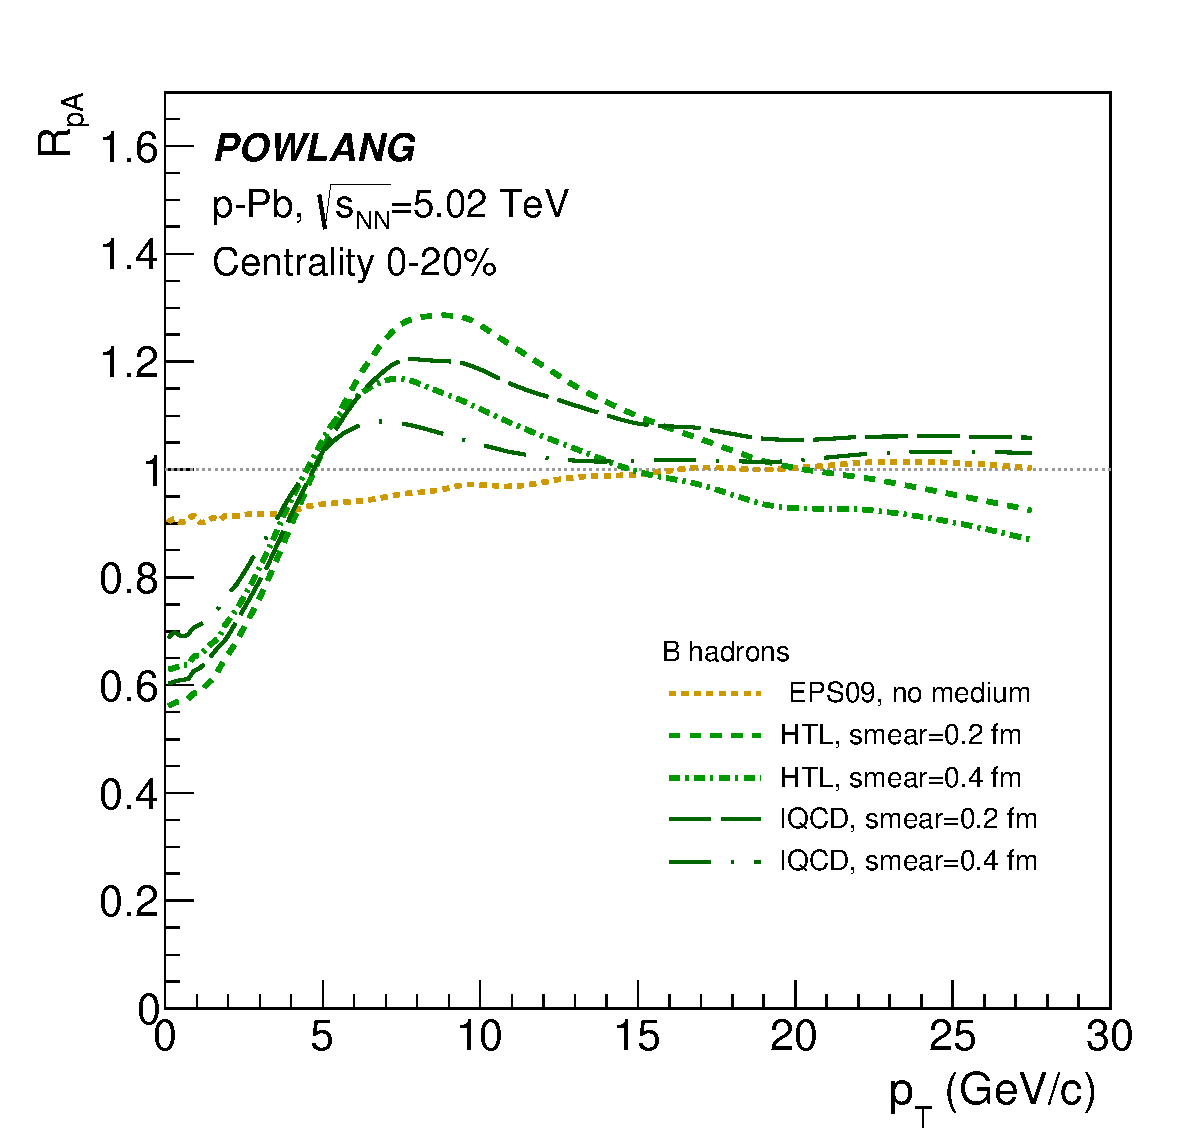
\includegraphics[width=0.4\textwidth]{hf/figures/Beauty-RpPb5TeV-HTLvsLat.pdf}
\caption{Left: Projection for the measurement of the nuclear modification factor of B mesons in \pPb collisions at $\sqrtsnn=5.02~\UTeV$ achievable by CMS with an integrated luminosity of 2 pb$^{-1}$.
Right: The nuclear modification factor of beauty hadrons in \pPb collisions at $\sqrtsnn=5.02$ TeV. Results of the POWLANG model with different choices of the transport coefficients and of the smearing of the initial condition are shown. Also reported, in yellow, the curve containing only Cold-Nuclear-Matter effect.}
\label{fig:POWLANG-small1}
\end{figure}
%%%%%%%%%%%%%%%%%%%%%%%%%%%%%%%%%%%%%%%%%%%%%%%%%%%%%%%
\begin{figure}[ht]
\centering
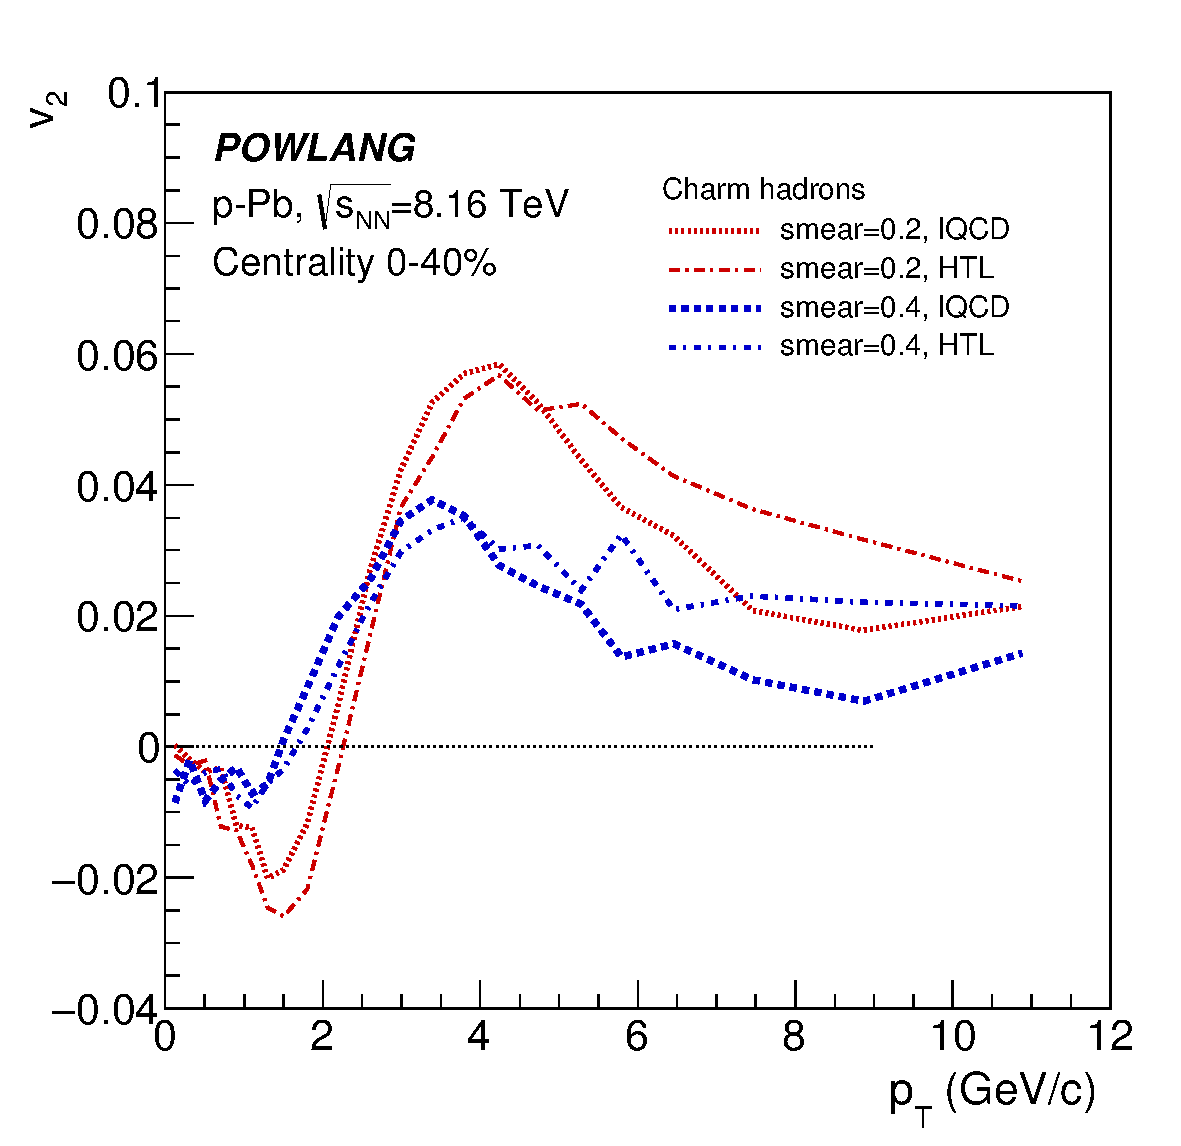
\includegraphics[width=0.4\textwidth]{hf/figures/v2cD_pPb8TeV_smear.pdf}
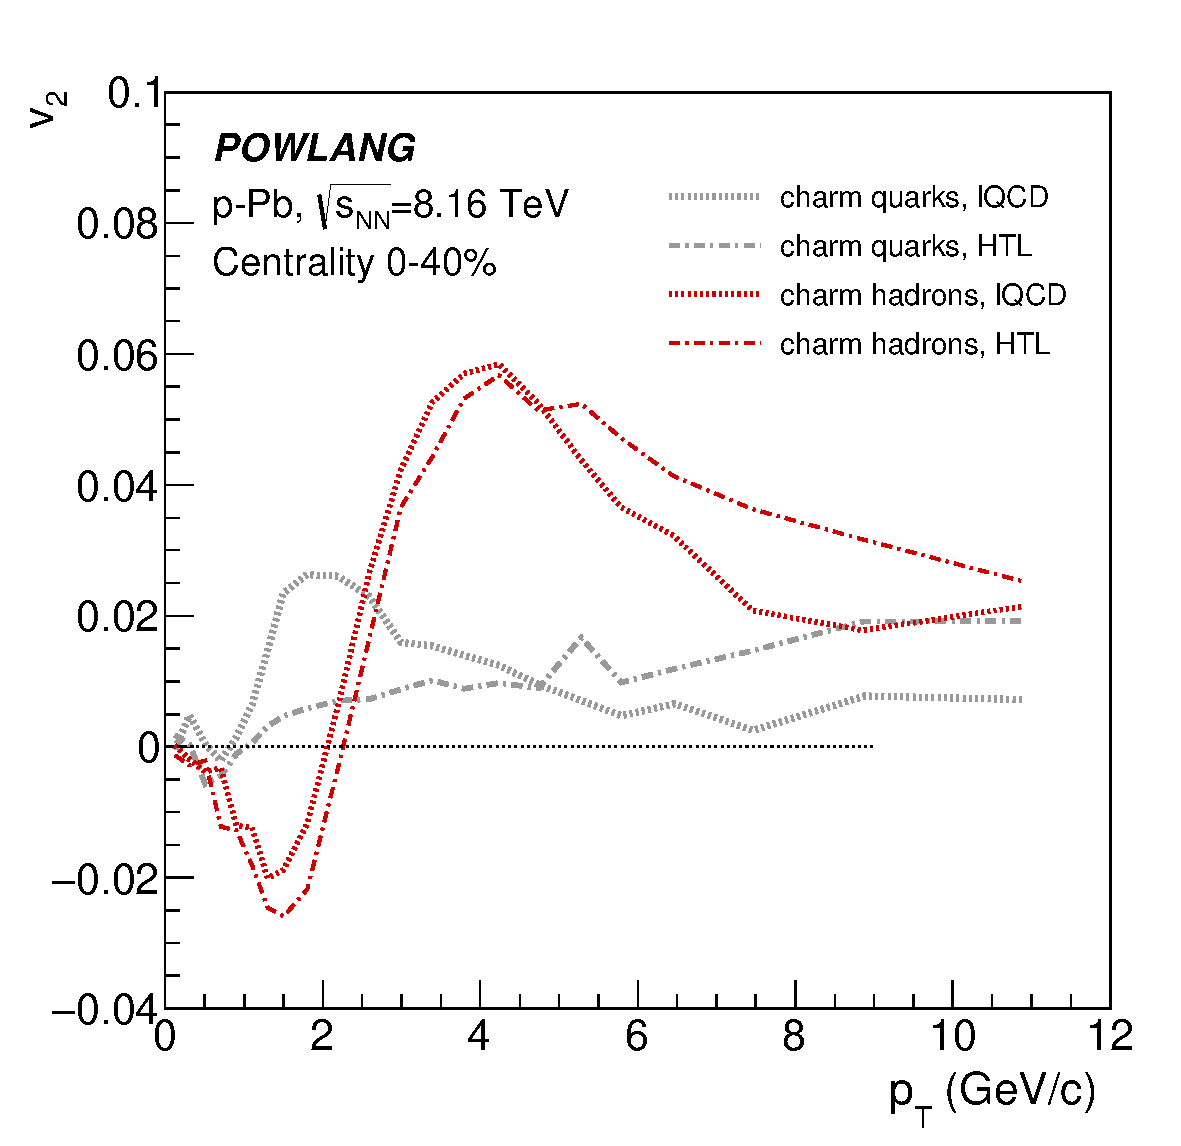
\includegraphics[width=0.4\textwidth]{hf/figures/v2cD_pPb8TeV_HTLvslQCD.pdf}
\caption{
Left: The elliptic flow of charmed hadrons in the 0-40\% most central \pPb collisions at $\sqrtsNN=8.16$~$\UTeV$. Results of the POWLANG model with different choices of the transport coefficients and of the smearing of the initial condition are shown. 
Right: a comparison of the results at the level of charm quarks and hadrons. An important fraction of the flow is acquired at hadronization via recombination with light partons from the medium.}
\label{fig:POWLANG-small2}
\end{figure}
%%%%%%%%%%%%%%%%%%%%%%%%%%%%%%%%%%%%%%%%%%
\begin{figure}[ht]
\centering
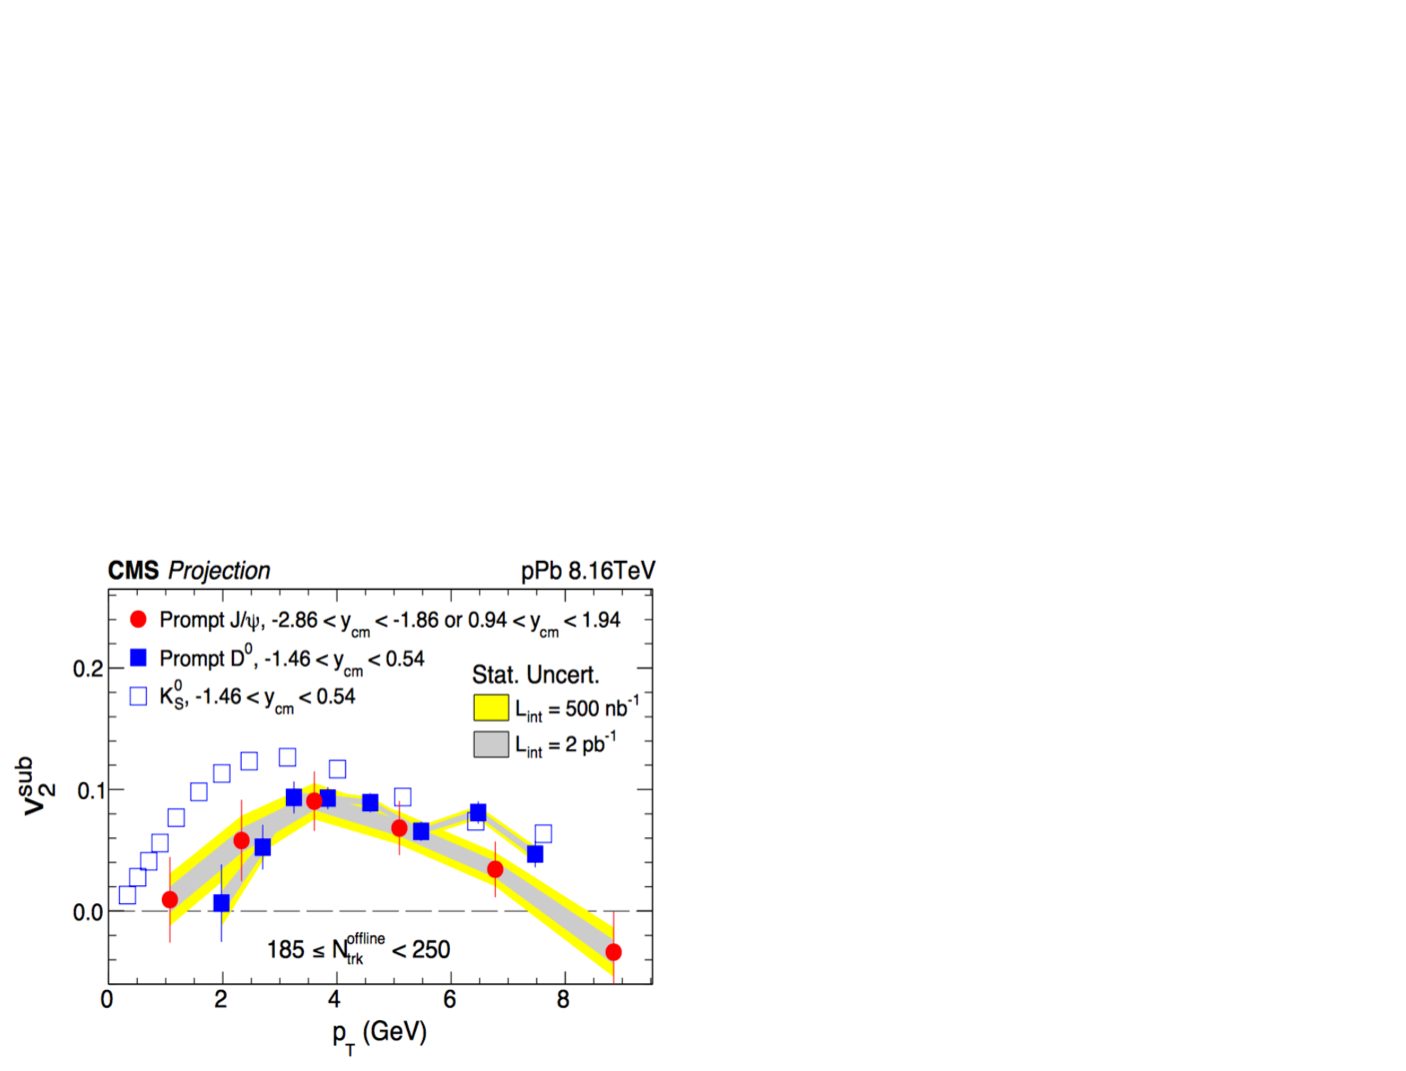
\includegraphics[width=0.4\textwidth]{hf/figures/CMS_Dv2.pdf}
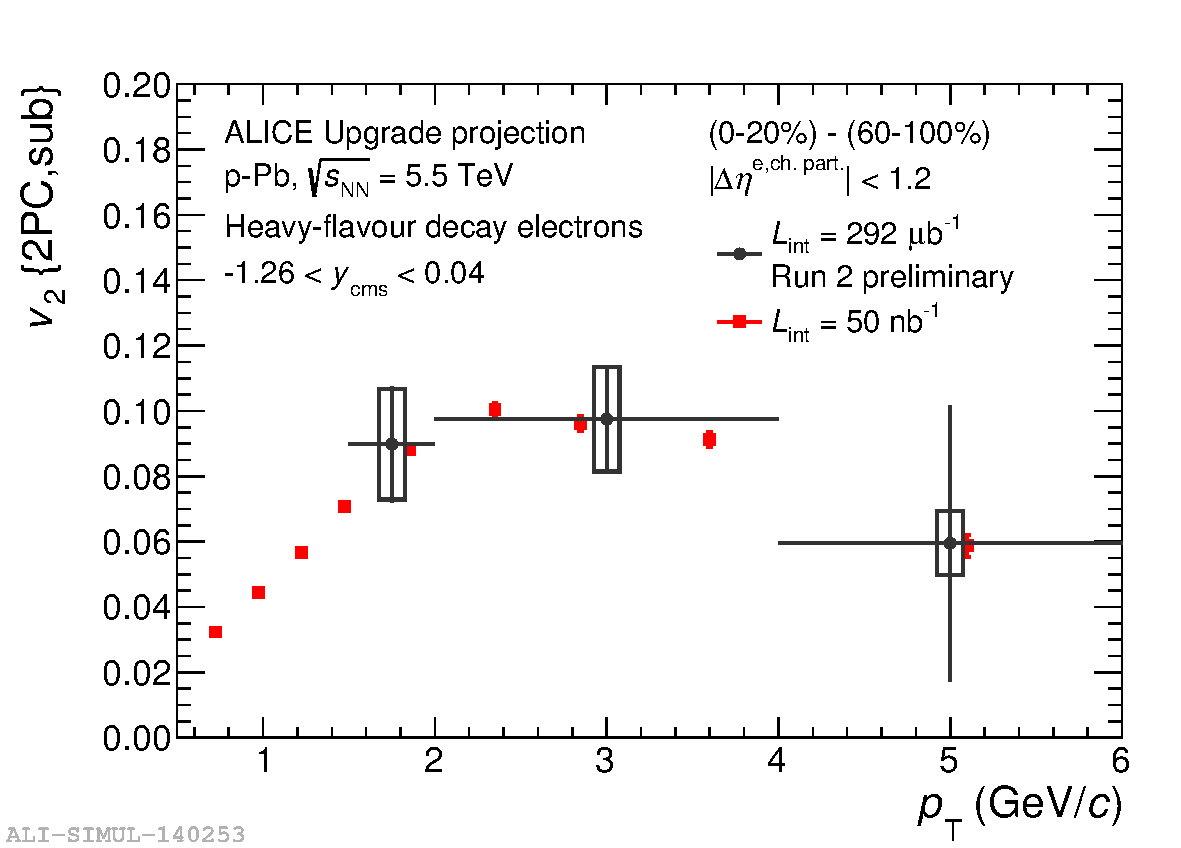
\includegraphics[width=0.43\textwidth]{hf/figures/2017-Oct-30-HFev2Plot.pdf}
\caption{
Left: projection of D-meson elliptic flow as a function of $\pt$ in high-multiplicity \pPb collisions at $\sqrtsNN=8.16$~$\UTeV$ with CMS.
Right: projection of elliptic flow of electrons from heavy-flavour hadron decays as a function of $\pt$ in 0--20\% central \pPb collisions at $\sqrtsNN=5.02$~$\UTeV$ with ALICE.}
\label{fig:elliptic-data}
\end{figure}
%%%%%%%%%%%%%%%%%%%%%%%%%
%%%%%%%%%%%%%%%%%
In order to illustrate the level of precision which future experimental measurements must reach to discriminate among different scenarios of initial and final-state effects, various sets of predictions based on the POWLANG model are reported in the following~\cite{Beraudo:2015wsd}.
In Fig.~\ref{fig:POWLANG-small1} (right) results of transport calculations for the nuclear modification factor of beauty hadrons in \pPb collisions at $\sqrtsnn=5.02~\UTeV$  are displayed and compared to experimental projections by CMS for the B-meson $R_{\rm pPb}$ (left) obtained from Run 2 data. As can be seen, model predictions are sensitive to the different choices of the transport coefficients (see discussion in~\cite{Beraudo:2015wsd}) and of the initial conditions (each nucleon-nucleon collision is assumed to deposit some entropy with a Gaussian smearing). In order to answer the question about possible final-state hot-medium effects, experimental measurements should be extended to lower $\pT$, as it is in program for the different experiments (see ALICE plans to perform beauty measurements down to low $\pT$ in nucleus-nucleus collisions in Sec.~\ref{sec:HFRAAv2}). In fact, for $\pT$ larger than 10--15~GeV/$c$ the curves accounting for the transport and hadronization of the heavy quarks in a hot medium (green curves) are very close to the (yellow) one which includes only the effect of the nPDF's and of the initial $k_{\rm T}$-broadening acquired in CNM, all of them being very close to unity as the experimental projections by CMS. On the contrary, at lower $\pT$ the radial flow of the beauty hadrons, acquired in part during the propagation through the hot medium and in part at hadronization via recombination, leads to a depletion of the spectrum at low $\pT$ and to an enhancement at intermediate $\pT$ which would allow one to distinguish this scenario from the case of pure CNM effects. 

As displayed in Fig.~\ref{fig:POWLANG-small2} the possible production of a hot deconfined medium in proton-nucleus collisions would also leave its fingerprints in the azimuthal distribution of the final hadrons, leading in particular to a non-vanishing elliptic-flow coefficient. Notice how one gets a positive $v_2$ for charmed hadrons only starting from $p_T\!\approx\!2$~GeV/$c$, in agreement with recent CMS data~\cite{Sirunyan:2018toe}. Differently from the heavy-ion case, in such small systems it is important how the initial entropy deposition is modelled with varying the smearing parameter (left panel). As displayed in the right panel of Fig.~\ref{fig:POWLANG-small2}, within the framework of the model, an important role is played by hadronization via recombination with light partons from the fireball, whose collective flow enhances the azimuthal asymmetry of the charmed hadrons.
%which reaches values comparable with the experimental observations shown -- together with the reduction of their statistical uncertainties as the integrated luminosity increases -- in Fig.~\ref{fig:elliptic-data}.

The projected precision with p--Pb integrated luminosities $\Lint\sim 2~\invpb$  (ATLAS and CMS) and $\sim 1$~pb$^{-1}$ (ALICE) has the potential to shed light on the different mechanisms behind the observed anisotropy (see Fig.~\ref{fig:elliptic-data} for D mesons with CMS and electrons from heavy-flavour hadron decays with ALICE).

%A complementary information is provided by charmonium measurements. Results on the elliptic flow of the J$/\psi$ in high-multiplicity \pPb collisions from ALICE~\cite{Acharya:2017tfn} and CMS~\cite{CMS:2018xac} start getting available, providing evidence for a positive $v_2$. In particular preliminary CMS data obtained in ``ultra-central'' events, also displayed in the left panel of Fig.~\ref{fig:elliptic-data},  show an elliptic flow of the J$/\psi$ comparable to the one of D mesons~\cite{CMS:2018xac}. This is clearly challenging from the point of view of the theoretical interpretation, since in the case of charmonium all the flow at the hadronic level must come from the one of the heavy quarks: either the coupling of the charm quarks with the produced medium is very strong or the origin of the positive $v_2$ must be looked for somewhere else, as pointed out in Ref.~\cite{Du:2018wsj} and already mentioned at the beginning of this section for the case of light hadrons.

Besides the analysis of kinematic distributions (in momentum and angle) of heavy-flavour particles, further interesting information on the onset of possible medium effects may come from the study of the yields of the various charm and beauty hadrons as a function of charged-particle multiplicity going from pp to \pPb and Pb--Pb, as done in the past for the case of strangeness production. As an example, with high-multiplicity triggers in pp collisions at $\sqrts =14$~$\UTeV$ ($L_{\rm int}=200$~pb$^{-1}$), the ALICE experiment will have the potential to detect D mesons with a precision better than 10\% in a wide kinematic range up to about 10--12 times the average charged-particle multiplicity. 


%\begin{itemize}
%\item{RpPb} (D, B, baryons): mid and fwd rapidity to constrain CNM/small QGP effects in wide kinematic range
%\item{v2}  in high-multiplicity pPb (D, HF-decay electrons and muons) to constrain initial final state effects
%\item{pp high-multiplicity} bridge between pp to PbPb to study HF production processes, onset of coalescence.
%Theory connection crucial
%\end{itemize}

%\textbf{FIGURES}:
%\begin{enumerate}
%\item D RpA (ALICE,CMS, LHCb, ATLAS)
%\item v2 in high mult pPb: CMS D0,  ALICE HF electrons, ATLAS D*
%\item D-meson yields in high multiplicity pp (ALICE)
%\item Theory predictions for v2 in high mult pp/pPb?
%\end{enumerate}



